\chapter{Introduction of emerging manufacturing technologies and novel materials for low-loss circuits' realization}\label{emerging}

\indent In this Chapter the application of emerging materials and manufacturing technologies for the realization of low loss microwave circuits in strip transmission line technique is considered and discussed. Application of various 3D printing technologies and dedicated materials are the subject of this study, including Fused Deposition Modeling (FDM) and Poly Jet Printing (PJP) as well as wide variety of conductive and dielectric materials.
\\
\indent Initially adopted for rapid prototyping to test the design before the final product development, additive manufacturing (AM) technologies have rapidly evolved toward the complete (one-pass) manufacturing of end-use components \cite{pieee_sorrentino}. This is due to significant development of the manufacturing equipment as well as material engineering. Recently also RF engineers have started to leverage AM technologies, including 3D printing, to develop the next generation of microwave and millimeter-wave devices aimed at several applications operating from hundreds of megahertz to hundreds of gigahertz, among which are millimeter-wave wireless and satellite communication systems and components such as waveguides, sensors, antennas, filters, power dividers, etc.. In such areas, AM offers several advantages such as design and geometrical flexibility of the circuits superior to conventional 2.5D techniques due to three-dimensional nature of the technology, near-net shape manufacturing, reduced tooling and fixtures, and almost no process waste. Moreover, another enabling advantage of AM processes is that it allows for the realization of multifunction parts, which means that several functionalities (electrical, thermal, or structural) are implemented in a single object. Finally, compared to conventional machining techniques, AM can be applied to produce custom microwave devices at reduced lead time and costs. 
\\
\indent The Author has experimentally investigated various additive manufacturing technologies and dedicated materials in terms of low-loss stripline microwave circuits realization as well as developed novel circuits taking advantage of the recent developments in technology and material engineering. The results of the conducted research have been a subject of one journal paper submitted to \textit{IEEE Transactions on Microwave Theory and Techniques} and three conference papers presented at \textit{International Conference on Electrical, Electronics and System Engineering (ICEESE'17)} and \textit{Electronic Components and Technology Conference (ECTC'18)}, all under the auspices of \textit{Institute of Electrical and Electronics Engineers}, which constitute the Chapter.
\\
\indent In Section \ref{iceese_graphene}, the applicability of additive manufacturing with conductive Polylactic Acid (PLA) based filament for the realization of low-loss suspended microstrip microwave circuits is investigated. Filament is used to 3D print a case which serve three major functions: provides mechanical enclosure and support for the circuit, provides appropriate elevation of the thin laminate with a circuit's pattern over the ground plane and can potentially serve as a ground plane. The influence of the bulk conductivity of the utilized filament on total losses within the structure has been studied. Moreover, an exemplary transmission line hosted in Fused Deposition Modelling (FDM) 3D printed case has been manufactured and measured. Graphene-enhanced PLA material having volume conductivity of $\sim$ 166 S/m has been used yielding total loss of $\sim$ 0.14 dB/cm/GHz while reference case with copper foil ground plane yields total loss of $\sim$ 0.04 dB/cm/GHz.
\\
\indent Following, in Section \ref{ectc_electr}, the realization of microwave circuits in suspended microstrip structure with a 3D printed conductive enclosure is presented. An example of a low-pass filter with a cut-off frequency of 2.5 GHz was designed, manufactured and measured. A Fused Deposition Modeling (FDM) type 3D printing and a conductive copper-based filament recently developed by Multi 3D featuring superior conductivity over BlackMagic 3D's Graphene-enhance PLA were employed to realize an enclosure serving both mechanical and electrical purposes. The influence of the ground plane conductivity on the total loss within the circuit was studied, and requirements for the conductive material properties were established. Moreover, the impact of the print parameters as well as the connection between microstrip line and SMA connectors were investigated. The obtained measurements proved that the proposed approach is of potential use for circuits and systems operating within low GHz frequency range.
\\
\indent Moreover, in Section \ref{ectc_df-poly}, an application of additive manufacturing technologies for realization of multilayer microwave circuits in microstrip transmission line technique is presented. An example of a second-order cascaded loops directional filter allowing to separate 2100 MHz Long-Term Evolution (LTE) band was designed in suspended microstrip technique with three metal layers, manufactured using a combination of PolyJet 3D printing with UV cured VeroWhitePlus polymer material and magnetron sputtering of copper, and assembled out of two parts using a “lego-like” process. The obtained results for the manufactured circuit were evaluated in terms of electrical performance and total power loss showing that the proposed approach is of potential use for circuits and systems operating within the microwave frequency range.
\\
\indent Finally, in Section \ref{tmtt_right_left}, a novel approach for the realization of high-performance coupled-line directional couplers in suspended stripline technique is proposed taking advantage of recent development in 3D printing technology. A third degree of freedom is introduced to a 2.5D structure allowing to combine the advantages of strip-transmission-line techniques, for which the circuit can still be considered as a quasi-planar structure, with the 3D printing flexibility of air layer thickness variation limited only by technological constraints. It is shown, that the proposed approach is well suitable for the realization of low-loss circuits, where tight coupling and superior performance and compactness are required. Moreover, it is shown that compensating elements, often required to improve couplers' performance, can easily be realized as a combination of a circuit's pattern and ground plane integrated 3D structures allowing for better circuit's volume utilization. An example of a 3-dB coupled-line directional coupler operating within the ISM 5.8 GHz band is designed, manufactured and measured for experimental verification. The obtained results have shown high electrical performance and low power losses of the circuit confirming the applicability of the proposed approach.

\cleardoublepage

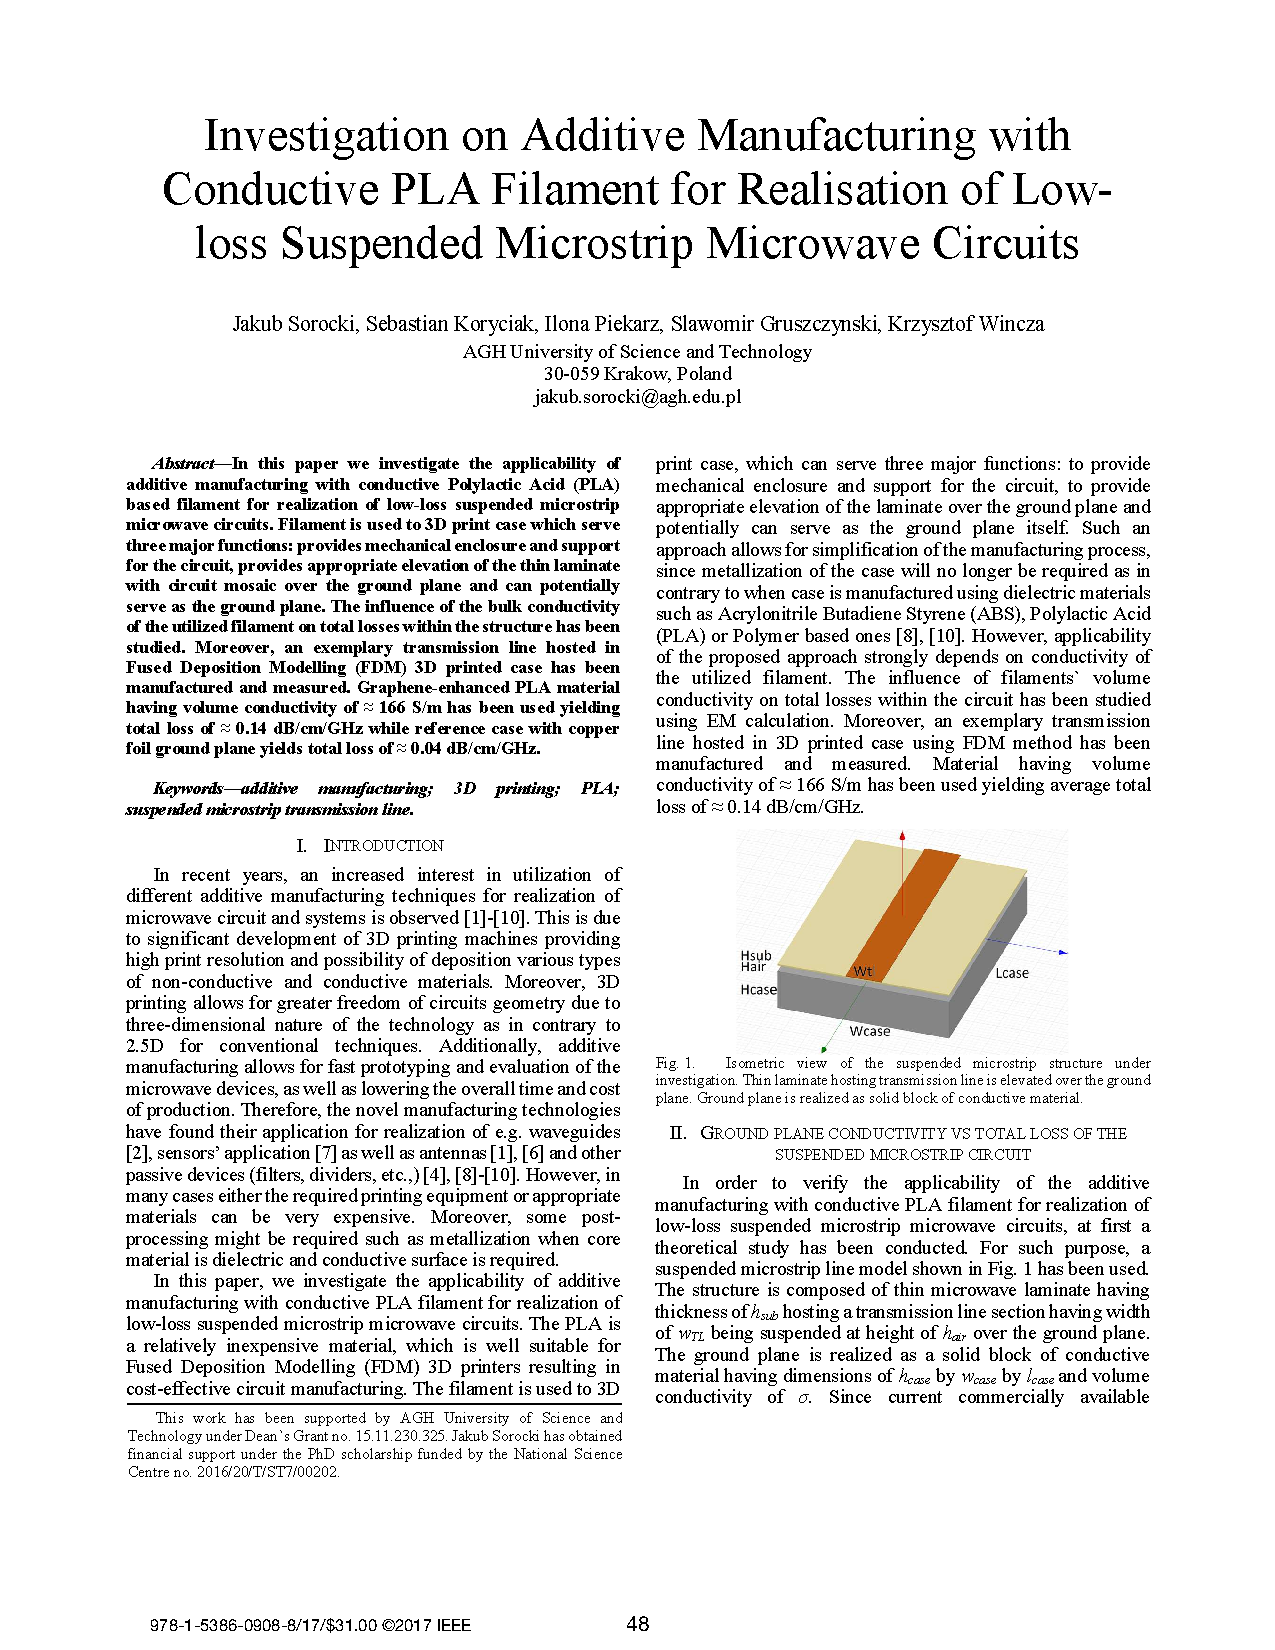
\includepdf[pages=-,addtotoc={1,section,1,Investigation on additive manufacturing with conductive PLA filament for realisation of low-loss suspended microstrip microwave circuits,iceese_graphene}, pagecommand={}, scale=.97]{chapter_5/iceese_graphene.pdf}

\cleardoublepage
 
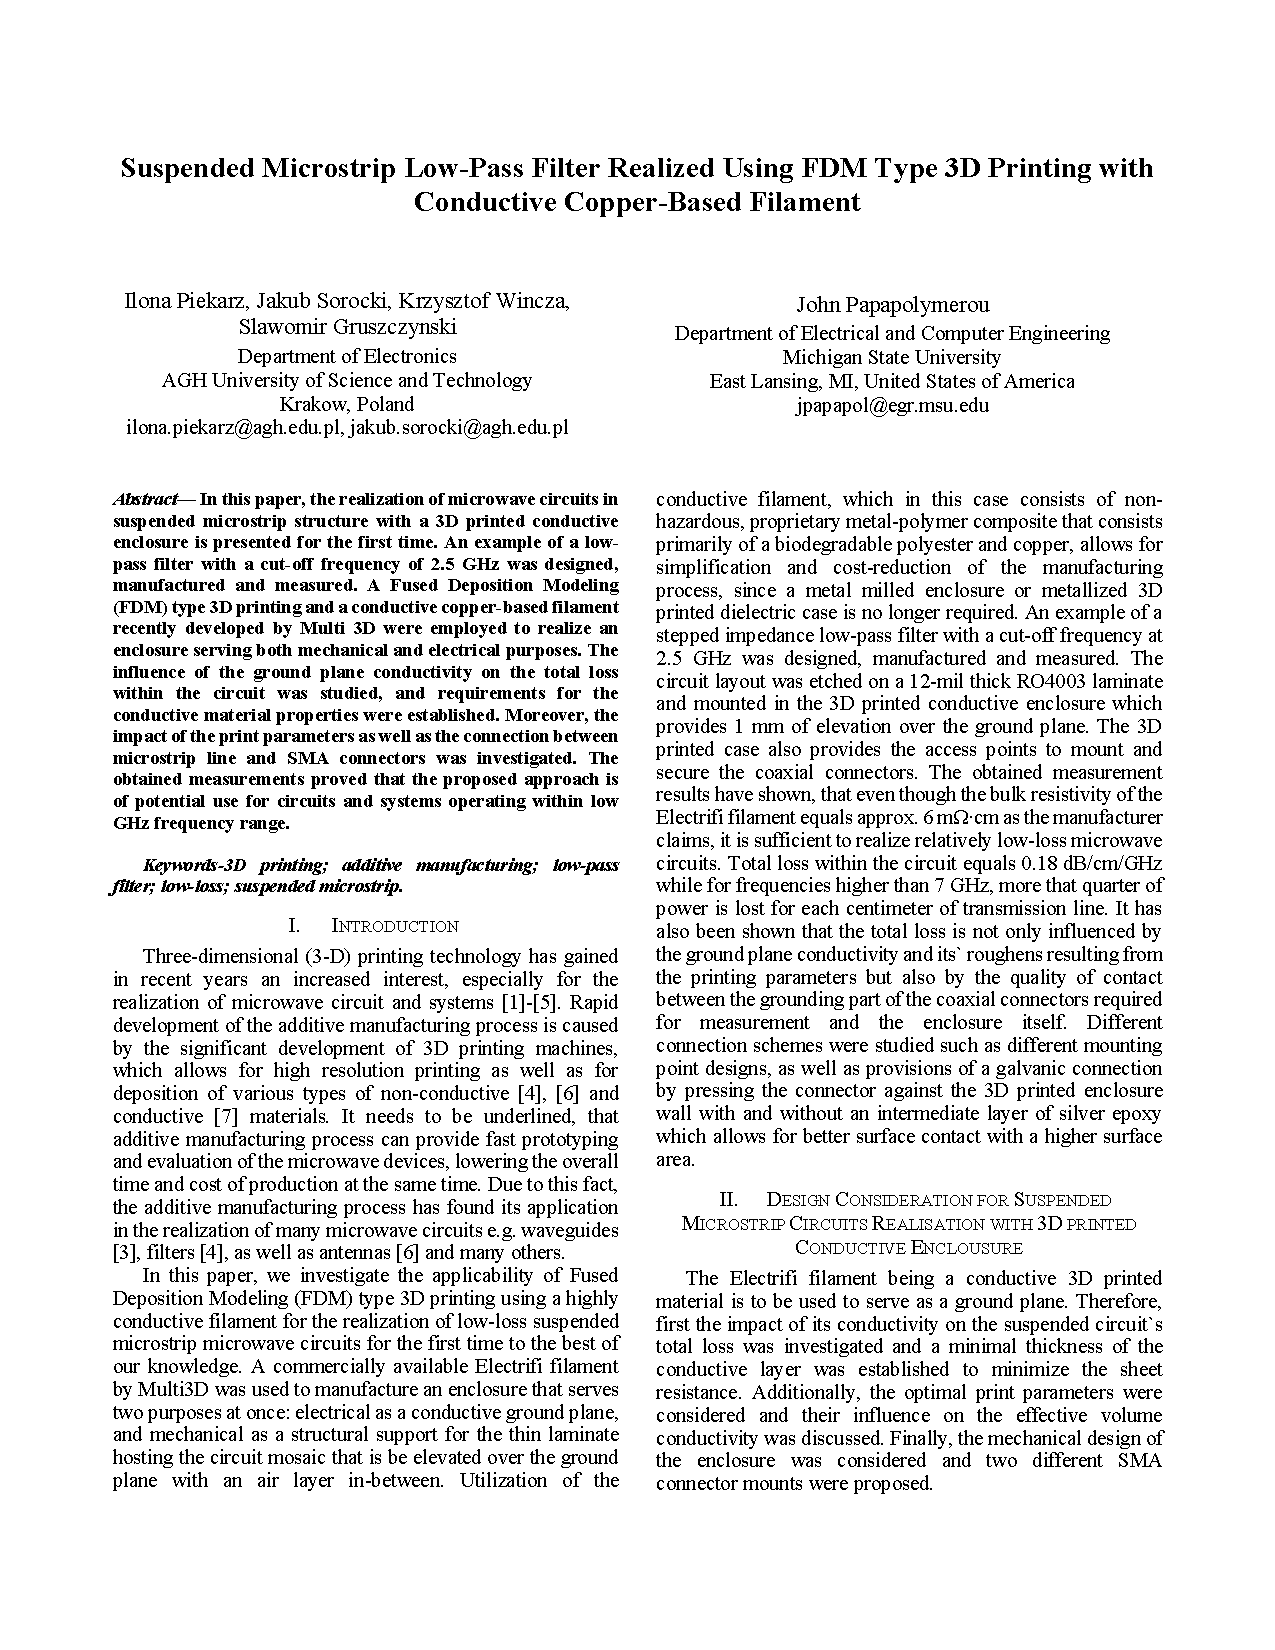
\includepdf[pages=-,addtotoc={1,section,1,Suspended microstrip low-pass filter realized using FDM type 3D printing with conductive copper-based filament,ectc_electr}, pagecommand={}, scale=.97]{chapter_5/ectc_electr.pdf}

\cleardoublepage

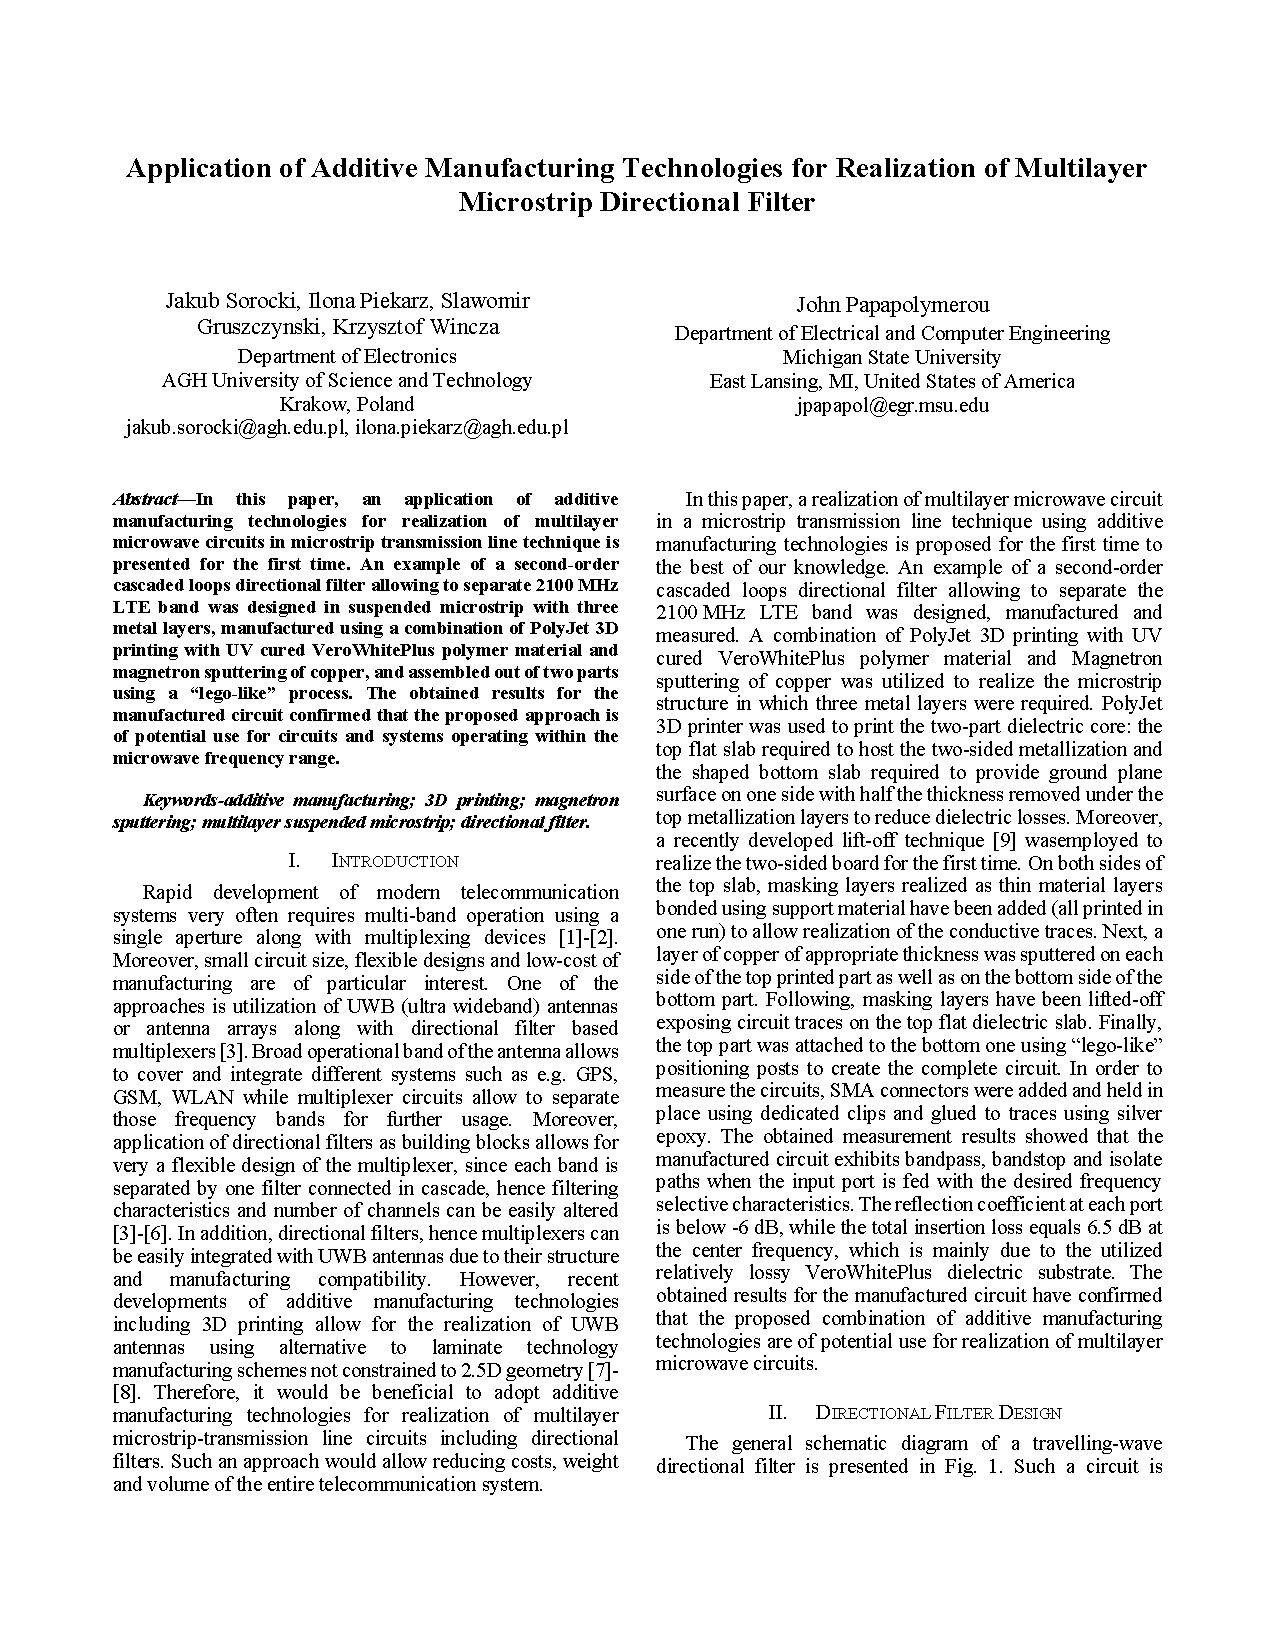
\includepdf[pages=-,addtotoc={1,section,1,Application of additive manufacturing technologies for realization of multilayer microstrip directional filter,ectc_df-poly}, pagecommand={}, scale=.97]{chapter_5/ectc_df-poly.pdf}

\cleardoublepage

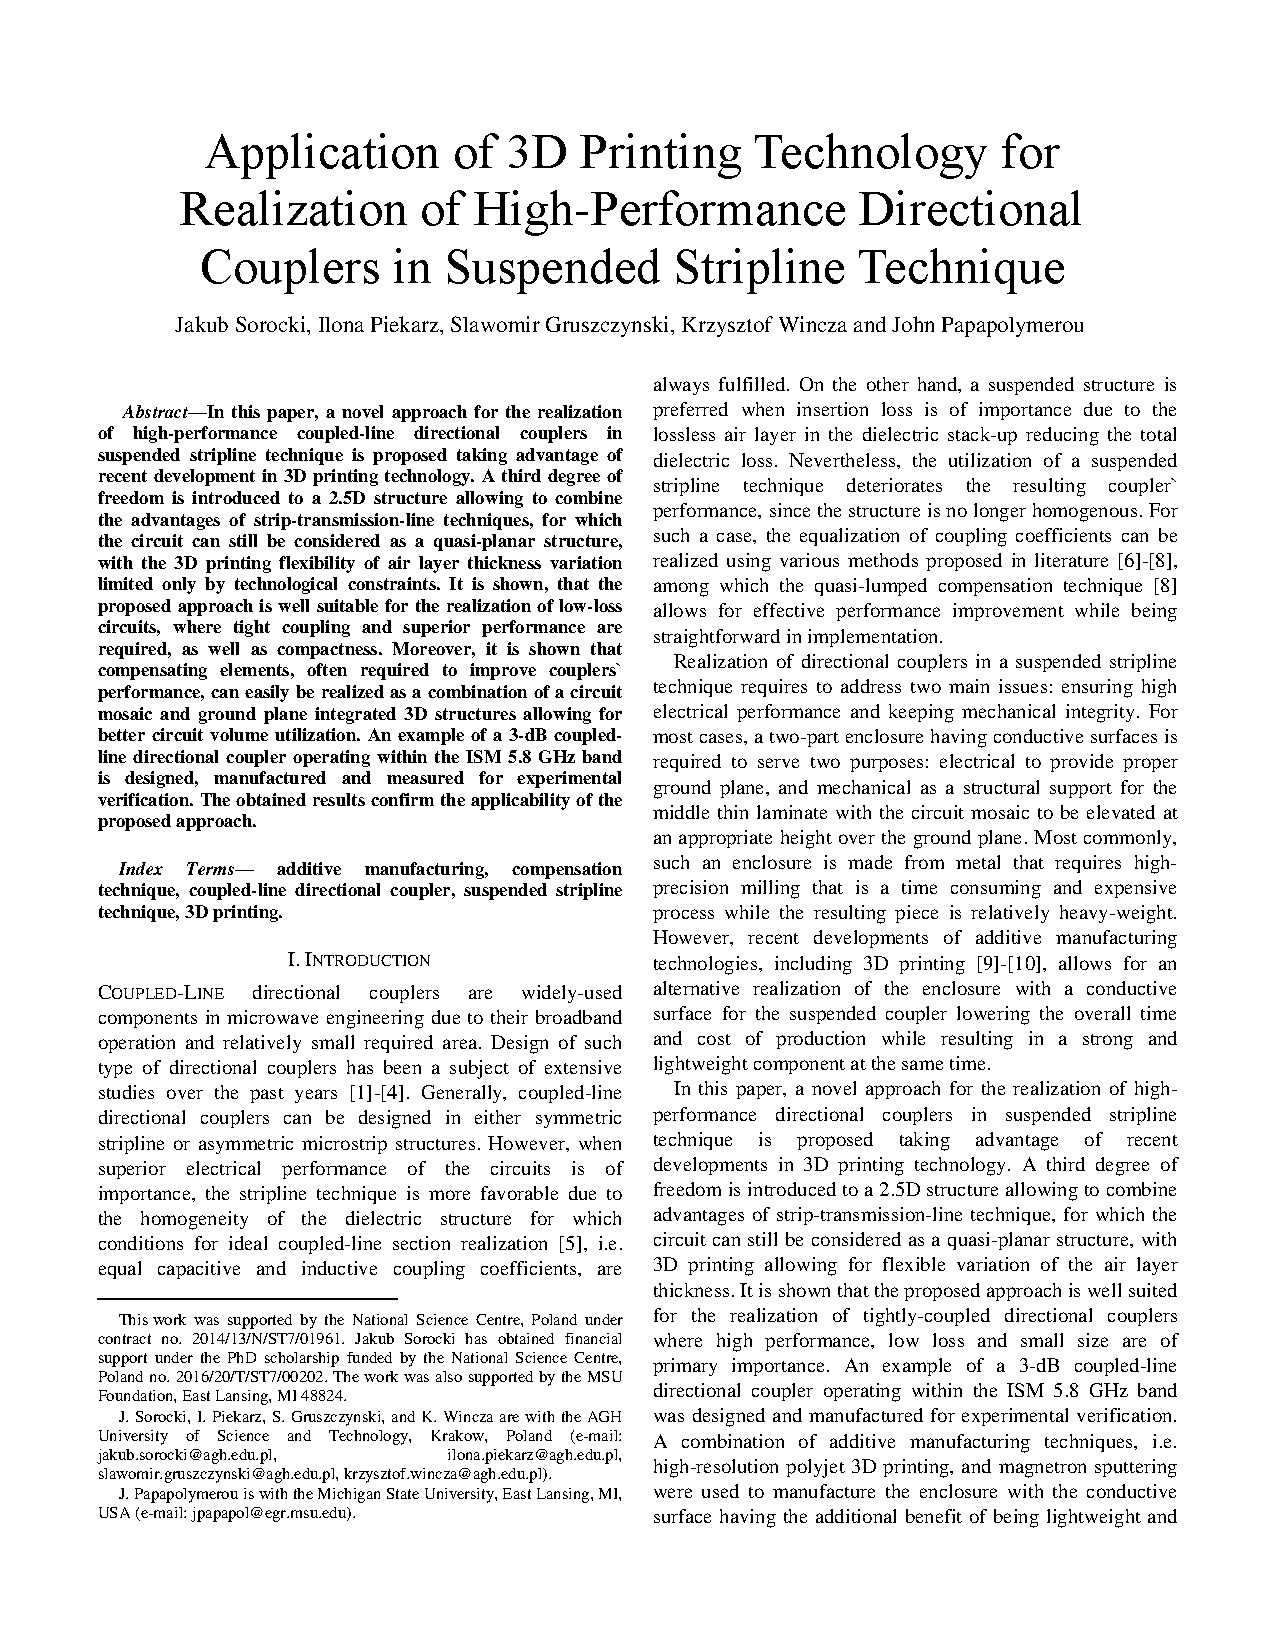
\includepdf[pages=-,addtotoc={1,section,1,Application of 3D printing technology for realization of high-performance directional couplers in suspended stripline technique,tmtt_right_left}, pagecommand={}, scale=.97]{chapter_5/polyjet_suspended_coupler.pdf}

\cleardoublepage